%%%%%%%%%%%%%%%%%%%%%%%%%%%%%%%%%%%%%%%%%
% Beamer Presentation
% LaTeX Template
% Version 1.0 (10/11/12)
%
% This template has been downloaded from:
% http://www.LaTeXTemplates.com
%
% License:
% CC BY-NC-SA 3.0 (http://creativecommons.org/licenses/by-nc-sa/3.0/)
%
%%%%%%%%%%%%%%%%%%%%%%%%%%%%%%%%%%%%%%%%%

%----------------------------------------------------------------------------------------
%	PACKAGES AND THEMES
%----------------------------------------------------------------------------------------

\documentclass{beamer}

\mode<presentation> {

% The Beamer class comes with a number of default slide themes
% which change the colors and layouts of slides. Below this is a list
% of all the themes, uncomment each in turn to see what they look like.

%\usetheme{default}
%\usetheme{AnnArbor}
%\usetheme{Antibes}
%\usetheme{Bergen}
%\usetheme{Berkeley}
%\usetheme{Berlin}
%\usetheme{Boadilla}
%\usetheme{CambridgeUS}
%\usetheme{Copenhagen}
%\usetheme{Darmstadt}
%\usetheme{Dresden}
%\usetheme{Frankfurt}
%\usetheme{Goettingen}
%\usetheme{Hannover}
%\usetheme{Ilmenau}
%\usetheme{JuanLesPins}
%\usetheme{Luebeck}
\usetheme{Madrid}
%\usetheme{Malmoe}
%\usetheme{Marburg}
%\usetheme{Montpellier}
%\usetheme{PaloAlto}
%\usetheme{Pittsburgh}
%\usetheme{Rochester}
%\usetheme{Singapore}
%\usetheme{Szeged}
%\usetheme{Warsaw}

% As well as themes, the Beamer class has a number of color themes
% for any slide theme. Uncomment each of these in turn to see how it
% changes the colors of your current slide theme.

%\usecolortheme{albatross}
%\usecolortheme{beaver}
%\usecolortheme{beetle}
%\usecolortheme{crane}
%\usecolortheme{dolphin}
%\usecolortheme{dove}
%\usecolortheme{fly}
%\usecolortheme{lily}
%\usecolortheme{orchid}
%\usecolortheme{rose}
%\usecolortheme{seagull}
%\usecolortheme{seahorse}
%\usecolortheme{whale}
%\usecolortheme{wolverine}

%\setbeamertemplate{footline} % To remove the footer line in all slides uncomment this line
%\setbeamertemplate{footline}[page number] % To replace the footer line in all slides with a simple slide count uncomment this line

%\setbeamertemplate{navigation symbols}{} % To remove the navigation symbols from the bottom of all slides uncomment this line
}

\usepackage{graphicx} % Allows including images
\usepackage{booktabs} % Allows the use of \toprule, \midrule and \bottomrule in tables

%----------------------------------------------------------------------------------------
%	TITLE PAGE
%----------------------------------------------------------------------------------------

\title[LiDAR]{Introduction to LiDAR} % The short title appears at the bottom of every slide, the full title is only on the title page

\author{Sanam Moslemi-Tabrizi} % Your name
\institute[] % Your institution as it will appear on the bottom of every slide, may be shorthand to save space
{
Carleton University \\ % Your institution for the title page
\medskip
\textit{smoslemi@yahoo.ca} % Your email address
}
\date{\today} % Date, can be changed to a custom date

\begin{document}

\begin{frame}
\titlepage % Print the title page as the first slide
\end{frame}

\begin{frame}
\frametitle{Overview} % Table of contents slide, comment this block out to remove it
\tableofcontents % Throughout your presentation, if you choose to use \section{} and \subsection{} commands, these will automatically be printed on this slide as an overview of your presentation
\end{frame}

%----------------------------------------------------------------------------------------
%	PRESENTATION SLIDES
%----------------------------------------------------------------------------------------

%------------------------------------------------
\section{Introduction} % Sections can be created in order to organize your presentation into discrete blocks, all sections and subsections are automatically printed in the table of contents as an overview of the talk
\begin{frame}
\frametitle{Introduction}
\begin{itemize}
\item Light Detection and Ranging (LIDAR) is a very accurate mapping technology.
\item A LiDAR device fires rapid pulses of laser light at a surface and a sensor on the device measures time of flight. By repeating this process, a complex map of the surface is built. 
\item The return light include noise. One method to reduce noise is to to put a signature on the transmitted light and detect only the returned signal with the signature.
\end{itemize}
\end{frame}
%
\section{Applications} 
\begin{frame}
\frametitle{Applications}
\begin{itemize}
\item Autonomous systems are a key market for LIDAR devices.
\item Robotics, Atmospheric measurement, Archeology
\item and even Forensics!
\end{itemize}
Wavelength categories:
\begin{itemize}
\item 600-1000nm lasers are more commonly used for non-scientific purposes but the maximum power has to be limited to make them eye-safe.
\item Lasers with a wavelength of 1550nm are used for longer range and lower accuracy purposes. This range does not show under night-vision goggles, therefore well suited to military applications.
\end{itemize}
\end{frame}
%


\begin{frame}
\frametitle{Basics (cont.)}
\begin{columns}[c] % The "c" option specifies centered vertical alignment while the "t" option is used for top vertical alignment

\column{.55\textwidth} % Left column and width
    \begin{figure}[htbp]
    \begin{center}
    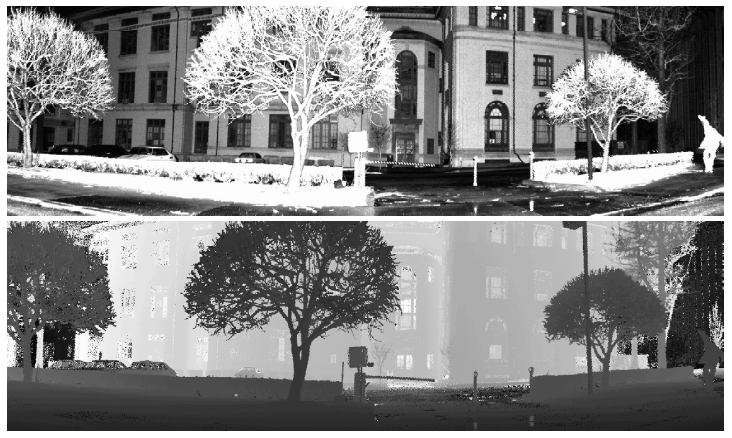
\includegraphics[width=6cm]{graphs/lidar_data}
    \caption{LiDAR data}
    \label{default}
    \end{center}
    \end{figure}

\column{.5\textwidth} % Right column and width
    \begin{figure}[htbp]
    \begin{center}
    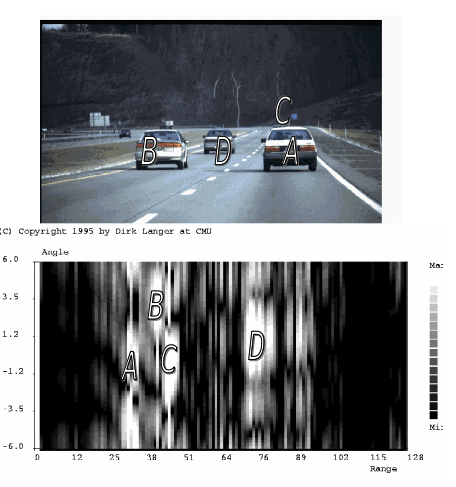
\includegraphics[width=6cm]{graphs/radar_data}
    \caption{RADAR data}
    \label{default}
    \end{center}
    \end{figure}

\end{columns}
\end{frame}

%\begin{itemize}
%\item Using proper modulation technique, it is possible the distance and velocity simultaneously \cite{pic0}.
%\item Beam steering in the key element of LiDAR systems.
%\end{itemize}

\begin{frame}
\frametitle{Basics}
\begin{columns}[c] % The "c" option specifies centered vertical alignment while the "t" option is used for top vertical alignment

\column{.55\textwidth} % Left column and width
\begin{itemize}
\item Tunable laser
\item Semiconductor optical amplifiers 
\item Splitters. MMI or Star coupler.
\item Thermo-optical phase modulators (mainly resistive thermo optic phase shifters)
\end{itemize}

\column{.5\textwidth} % Right column and width
   \begin{figure}[htbp]
    \begin{center}
    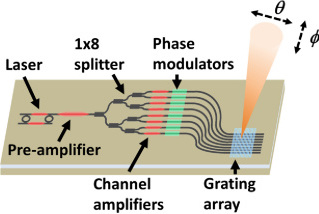
\includegraphics[width=6cm]{graphs/pic3}
    \caption{An example LiDAR system \cite{pic3}}
    \label{default}
    \end{center}
    \end{figure}

\end{columns}
\end{frame}
%
\begin{frame}
\frametitle{Basics (cont.)}
\begin{columns}[c] % The "c" option specifies centered vertical alignment while the "t" option is used for top vertical alignment

\column{.55\textwidth} % Left column and width
\begin{itemize}
\item Channels and spacing
    \begin{itemize}
    \item The angular separation between the main lobe and the side lobes ($\phi$) is defined by spacing d: d$\searrow \;  \; \Rightarrow \;  \; \phi \; \nearrow$
    \item The peak power of the side lobes is also a function of the ratio output waveguide width to channel d$\searrow \;  \; \Rightarrow \;  \;$ peak power  $\nearrow$
    \item Very small spacing will cause crosstalk between channels
    \item Non-uniform spacing \cite{pic2}
    \end{itemize}
\item Surface grating (pitch of 0.55 $\mu m$ nd a duty of 20$\%$)
\end{itemize}

\column{.45\textwidth} % Right column and width
\begin{figure}[htbp]
    \begin{center}
    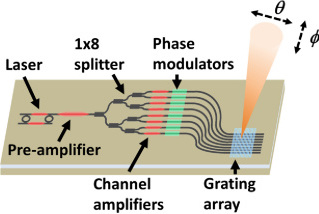
\includegraphics[width=5cm]{graphs/pic3}
    \caption{An example LiDAR system \cite{pic3}}
    \label{default}
    \end{center}
    \end{figure}

\end{columns}
\end{frame}

%
\section{Beam steering} 
\begin{frame}
\frametitle{Beam steering}
\begin{itemize}
\item By tuning wavelength, the beam in the far field can be steered in one axis ($\theta$)
    \begin{equation}
    \sin(\theta)\, =\, \frac{\Lambda n_{eff} - \lambda}{\Lambda }
    \end{equation}
\item The relative phase across the grating array determines the beam shape/direction in the other axis ($\phi$)
\end{itemize}

\begin{figure}[htbp]
    \begin{center}
    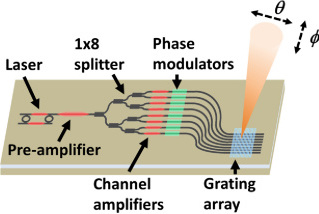
\includegraphics[width=8cm]{graphs/pic3}
%    \caption{An example LiDAR system \cite{pic3}}
    \label{default}
    \end{center}
    \end{figure}
 \end{frame}
%
\section{Examples} 
\begin{frame}
\frametitle{Another example}
    \begin{figure}[htbp]
    \begin{center}
    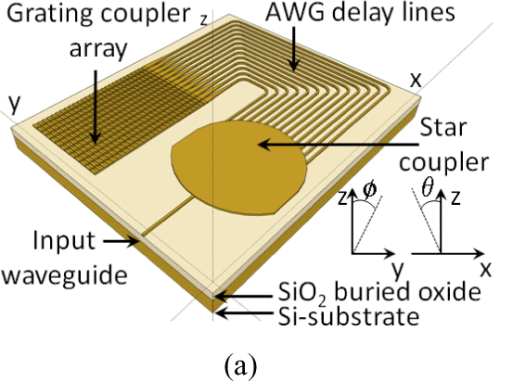
\includegraphics[width=6cm]{graphs/pic6_6}
    \caption{An example LiDAR system \cite{pic6_opa}}
    \label{default}
    \end{center}
    \end{figure}
\end{frame}
\begin{frame}
    \begin{figure}[htbp]
    \begin{center}
    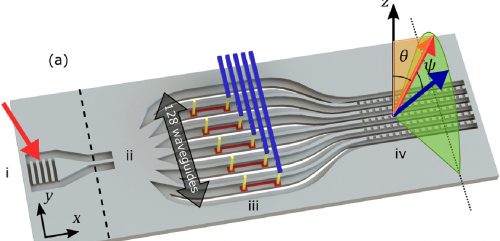
\includegraphics[width=8cm]{graphs/pic2}
    \caption{An example LiDAR system \cite{pic2}}
    \label{default}
    \end{center}
    \end{figure}
\end{frame}
\begin{frame}
\frametitle{Another example}
    \begin{figure}[htbp]
    \begin{center}
    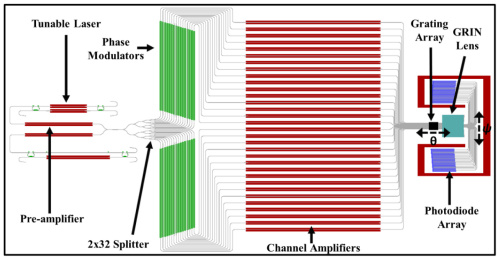
\includegraphics[width=10cm]{graphs/pic4}
    \caption{An example LiDAR system \cite{pic4}}
    \label{default}
    \end{center}
    \end{figure}
\end{frame}
%
\begin{frame}
\frametitle{MIT example}
\begin{columns}[c] % The "c" option specifies centered vertical alignment while the "t" option is used for top vertical alignment

\column{.7\textwidth} % Left column and width
\begin{itemize}
\item A LiDAR instrument with silicon photonic optical phased arrays.
\item FMCW LIDAR allows for simultaneous Doppler-based velocity measurements.
\item Triangular modulation is used to help with distance/velocity measurements.
\item The time delay between RX and LO will create an electrical beat frequency.
\item For a stationary target, this frequency is proportional to the distance of the target
\item For a moving target, because of the Doppler shift on RX we will get two beat frequencies
\item The difference of the two frequencies is twice the induced Doppler shift which is proportional to target's velocity.
\end{itemize}
\column{.4\textwidth} % Right column and width
   \begin{figure}[htbp]
    \begin{center}
    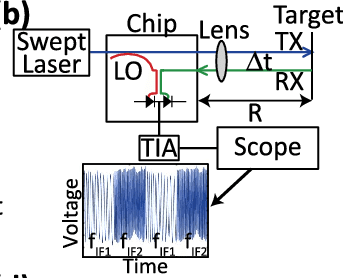
\includegraphics[width=4cm]{graphs/pic0}
    \caption{\cite{pic0}}
    \label{default}
    \end{center}
    \end{figure}

\end{columns}

\end{frame}



%------------------------------------------------

%\subsection{FMCW LIDAR with Triangular Modulation} % A subsection can be created just before a set of slides with a common theme to further break down your presentation into chunks

%\begin{frame}
%\frametitle{FMCW LiDAR}
%\begin{itemize}
%\itemThis system was fabricated within a 300 mm wafer CMOS compatible platform (low cost, can be integrated with CMOS Electronics). 
%\item Integrated optical phased arrays with solid-state beam steering.
%\item LiDAR than detect smaller objects with high resolution.
%\item Using proper modulation technique, it is possible the distance and velocity simultaneously \cite{pic0}.
%\item Beam steering in the key element of LiDAR systems.
%\end{itemize}
%\end{frame}

%\begin{frame}
%\frametitle{Paragraphs of Text}
%Sed iaculis dapibus gravida. Morbi sed tortor erat, nec interdum arcu. Sed id lorem lectus. Quisque viverra augue id sem ornare non aliquam nibh tristique. Aenean in ligula nisl. Nulla sed tellus ipsum. Donec vestibulum ligula non lorem vulputate fermentum accumsan neque mollis.\\~\\
%
%Sed diam enim, sagittis nec condimentum sit amet, ullamcorper sit amet libero. Aliquam vel dui orci, a porta odio. Nullam id suscipit ipsum. Aenean lobortis commodo sem, ut commodo leo gravida vitae. Pellentesque vehicula ante iaculis arcu pretium rutrum eget sit amet purus. Integer ornare nulla quis neque ultrices lobortis. Vestibulum ultrices tincidunt libero, quis commodo erat ullamcorper id.
%\end{frame}
%
%%------------------------------------------------
%
%\begin{frame}
%\frametitle{Bullet Points}
%\begin{itemize}
%\item Lorem ipsum dolor sit amet, consectetur adipiscing elit
%\item Aliquam blandit faucibus nisi, sit amet dapibus enim tempus eu
%\item Nulla commodo, erat quis gravida posuere, elit lacus lobortis est, quis porttitor odio mauris at libero
%\item Nam cursus est eget velit posuere pellentesque
%\item Vestibulum faucibus velit a augue condimentum quis convallis nulla gravida
%\end{itemize}
%\end{frame}
%
%%------------------------------------------------
%
%\begin{frame}
%\frametitle{Blocks of Highlighted Text}
%\begin{block}{Block 1}
%Lorem ipsum dolor sit amet, consectetur adipiscing elit. Integer lectus nisl, ultricies in feugiat rutrum, porttitor sit amet augue. Aliquam ut tortor mauris. Sed volutpat ante purus, quis accumsan dolor.
%\end{block}
%
%\begin{block}{Block 2}
%Pellentesque sed tellus purus. Class aptent taciti sociosqu ad litora torquent per conubia nostra, per inceptos himenaeos. Vestibulum quis magna at risus dictum tempor eu vitae velit.
%\end{block}
%
%\begin{block}{Block 3}
%Suspendisse tincidunt sagittis gravida. Curabitur condimentum, enim sed venenatis rutrum, ipsum neque consectetur orci, sed blandit justo nisi ac lacus.
%\end{block}
%\end{frame}
%
%%------------------------------------------------
%
%\begin{frame}
%\frametitle{Multiple Columns}
%\begin{columns}[c] % The "c" option specifies centered vertical alignment while the "t" option is used for top vertical alignment
%
%\column{.45\textwidth} % Left column and width
%\textbf{Heading}
%\begin{enumerate}
%\item Statement
%\item Explanation
%\item Example
%\end{enumerate}
%
%\column{.5\textwidth} % Right column and width
%Lorem ipsum dolor sit amet, consectetur adipiscing elit. Integer lectus nisl, ultricies in feugiat rutrum, porttitor sit amet augue. Aliquam ut tortor mauris. Sed volutpat ante purus, quis accumsan dolor.
%
%\end{columns}
%\end{frame}
%
%%------------------------------------------------
%\section{Second Section}
%%------------------------------------------------
%
%\begin{frame}
%\frametitle{Table}
%\begin{table}
%\begin{tabular}{l l l}
%\toprule
%\textbf{Treatments} & \textbf{Response 1} & \textbf{Response 2}\\
%\midrule
%Treatment 1 & 0.0003262 & 0.562 \\
%Treatment 2 & 0.0015681 & 0.910 \\
%Treatment 3 & 0.0009271 & 0.296 \\
%\bottomrule
%\end{tabular}
%\caption{Table caption}
%\end{table}
%\end{frame}
%
%%------------------------------------------------
%
%\begin{frame}
%\frametitle{Theorem}
%\begin{theorem}[Mass--energy equivalence]
%$E = mc^2$
%\end{theorem}
%\end{frame}
%
%%------------------------------------------------
%
%\begin{frame}[fragile] % Need to use the fragile option when verbatim is used in the slide
%\frametitle{Verbatim}
%\begin{example}[Theorem Slide Code]
%\begin{verbatim}
%\begin{frame}
%\frametitle{Theorem}
%\begin{theorem}[Mass--energy equivalence]
%$E = mc^2$
%\end{theorem}
%\end{frame}\end{verbatim}
%\end{example}
%\end{frame}
%
%%------------------------------------------------
%
%\begin{frame}
%\frametitle{Figure}
%Uncomment the code on this slide to include your own image from the same directory as the template .TeX file.
%%\begin{figure}
%%\includegraphics[width=0.8\linewidth]{test}
%%\end{figure}
%\end{frame}
%
%%------------------------------------------------
%
%\begin{frame}[fragile] % Need to use the fragile option when verbatim is used in the slide
%\frametitle{Citation}
%An example of the \verb|\cite| command to cite within the presentation:\\~
%
%This statement requires citation \cite{p1}.
%\end{frame}
%
%%------------------------------------------------

\begin{frame}
\frametitle{References}
\footnotesize{
\begin{thebibliography}{99} % Beamer does not support BibTeX so references must be inserted manually as below
\bibitem[J. K. Doylend, 2014]{pic4} J. K. Doylend, M. J. R. Heck, J. T. Bovington, J. D. Peters,M. L. Davenport (2014)
\newblock Fully integrated hybrid silicon free-space beam steering source with 32 channel phased array
%\newblock \emph{Journal Name} 12(3), 45 -- 678.
%
\bibitem[J. K. Doylend, 2013]{pic3} J. C. Hulme, J. K. Doylend, M. J. R. Heck, J. D. Peters, M. L. Davenport, J. T. Bovington, L. A. Coldren, and J. E. Bowers(2013)
\newblock Hybrid silicon free-space source with integrated beam steering
%\newblock \emph{Journal Name} 12(3), 45 -- 678.
%
\bibitem[Christopher V.  Poulton,2017]{pic0} Christopher V.  Poulton, Ami Yaacobi,  Davis B. Cole, Mathew J. Byrd,  Manan Raval, Dierdrik Vermeulen,  and Michael R. Watts (2017)
\newblock Coherent solid-state LIDAR with silicon photonic optical phased arrays
%\newblock \emph{Journal Name} 12(3), 45 -- 678.
%
\bibitem[Wim Bogaerts, 2011]{pic6_opa} Karel Van Acoleyen, Wim Bogaerts, and Roel Baets, (2011)
\newblock Two-Dimensional Dispersive Off-Chip Beam Scanner Fabricated on Silicon-On-Insulator
%\newblock \emph{Journal Name} 12(3), 45 -- 678.
%
\bibitem[David N. Hutchison, 2016]{pic2} David N. Hutchison, Jie Sun, Jonathan K. Doylend, Ranjeet Kumar, John Heck, Woosung Kim, Christopher T. Phare, Avi Feshali, and Haisheng Rong, (2016)
\newblock High-resolution aliasing-free optical beam steering
%\newblock \emph{Journal Name} 12(3), 45 -- 678.
\end{thebibliography}
}
\end{frame}

%------------------------------------------------

\begin{frame}
\Huge{\centerline{The End}}
\end{frame}

%----------------------------------------------------------------------------------------

\end{document} 